\documentclass[11pt,a4paper]{article}

% ----------------------------------------------------------------------
% AgriAssist — Project Report (Overleaf-ready, compile with pdfLaTeX)
% ----------------------------------------------------------------------
\usepackage[utf8]{inputenc}
\usepackage[T1]{fontenc}
\usepackage{lmodern}
\usepackage[a4paper,margin=1in]{geometry}
\usepackage{amsmath,amssymb}
\usepackage{graphicx}
\usepackage{booktabs}
\usepackage{array}
\usepackage{xcolor}
\usepackage{enumitem}
\usepackage{caption}
\usepackage{subcaption}
\usepackage{titlesec}
\usepackage{fancyhdr}
\usepackage{tikz}
\usepackage{pgfplots}
\pgfplotsset{compat=1.17}
\usetikzlibrary{positioning,arrows.meta,calc,fit,backgrounds}
\usepackage[hidelinks,colorlinks=true,linkcolor=forest,urlcolor=ochre,citecolor=forest]{hyperref}

% ---------------- palette ----------------
\definecolor{forest}{RGB}{35,78,55}
\definecolor{forestd}{RGB}{19,35,26}
\definecolor{moss}{RGB}{124,154,78}
\definecolor{mosslt}{RGB}{200,214,170}
\definecolor{ochre}{RGB}{198,138,30}
\definecolor{terra}{RGB}{168,70,46}
\definecolor{slate}{RGB}{78,124,134}
\definecolor{paper}{RGB}{247,246,240}
\definecolor{inkt}{RGB}{27,42,29}

% ---------------- section styling ----------------
\titleformat{\section}{\color{forest}\Large\bfseries}{\thesection}{0.6em}{}
\titleformat{\subsection}{\color{forestd}\large\bfseries}{\thesubsection}{0.6em}{}
\titlespacing*{\section}{0pt}{1.4em}{0.6em}
\pagestyle{fancy}\fancyhf{}
\lhead{\small\color{forest}\textbf{AgriAssist}}
\rhead{\small\color{inkt} CSIRO Pasture Biomass + Agentic Farm Assistant}
\cfoot{\small\thepage}
\renewcommand{\headrulewidth}{0.4pt}

% ---------------- tikz styles ----------------
\tikzset{
  proc/.style={rectangle, rounded corners=4pt, draw=forest, fill=forest!8,
    align=center, minimum height=1.05cm, inner sep=5pt, font=\footnotesize},
  procf/.style={proc, fill=forest, text=white, draw=forest},
  procm/.style={proc, fill=moss!30, draw=moss},
  proco/.style={proc, fill=ochre!18, draw=ochre},
  procs/.style={proc, fill=slate!18, draw=slate},
  proct/.style={proc, fill=terra!15, draw=terra},
  io/.style={proc, fill=mosslt!60, draw=moss},
  fl/.style={-{Stealth[length=2.2mm]}, thick, draw=ochre!80!black},
}
\newcommand{\R}{\mathbb{R}}
\setlength{\parskip}{0.4em}
\setlength{\parindent}{0pt}

% ======================================================================
\begin{document}

% ---------------- title page ----------------
\begin{titlepage}
\centering
\vspace*{1.5cm}
{\color{ochre}\large\bfseries ML COURSE PROJECT \quad\textbullet\quad PROBLEM BY CSIRO}\\[1.4cm]
{\color{forestd}\fontsize{46}{50}\selectfont\bfseries AgriAssist}\\[0.3cm]
{\color{forest}\Large\itshape The AI expert every farmer deserves}\\[1.0cm]
\rule{0.55\textwidth}{1.2pt}\\[0.7cm]
{\large A pasture-biomass estimator for the CSIRO problem, a district crop-yield\\
regressor and a soil-profile clusterer, unified by an agentic assistant that\\
remembers one Indian farm and answers by text, voice or photo.}\\[2.2cm]

\begin{tabular}{rl}
\textbf{Problem by} & Commonwealth Scientific and Industrial Research Organisation (CSIRO)\\[2pt]
\textbf{Course} & Introduction to Machine Learning\\[2pt]
\textbf{Team} & Sudhanshu \textit{(and team)}\\[2pt]
\textbf{Date} & \today\\
\end{tabular}

\vfill
{\small\color{gray} Pasture biomass $\cdot$ District crop yield $\cdot$ Soil profile clustering $\cdot$ LangGraph agent}
\end{titlepage}

% ---------------- abstract + toc ----------------
\begin{abstract}
\noindent
AgriAssist is an agentic artificial-intelligence agronomist for Indian farmers. A person
describes their farm once and then converses with an agent by text, voice or photograph.
Three trained machine-learning models sit at its core. A \emph{pasture-biomass} estimator
answers the CSIRO challenge of predicting the dry weight of feed from a single photograph; its
final architecture is a two-stream ResNet-50 whose embeddings are concatenated with twelve
hand-crafted green-vegetation statistics and read by five independent gradient-boosted
regressors. A \emph{crop-yield} model is a random forest over the recent district harvest record
for rice, wheat and maize. A \emph{soil-profile} model clusters six-number soil tests with
$k$-means. This report presents the problem framing, the data, the mathematics of each model,
the experiments that led to the final designs (including a diverged transformer baseline and a
Grad-CAM sanity check), the honest evaluation of each, and the LangGraph agent, twelve-tool
interface and three-tier memory that turn these numbers into farming decisions.
\end{abstract}

{\small\tableofcontents}
\newpage

% ======================================================================
\section{Introduction}
A farmer does not want a model score; they want a decision: graze or rest the field, sow or
wait, sell the crop or hold it. AgriAssist keeps a farm's facts (place, land, crops, animals,
soil, irrigation, goals) and answers in the language the person just used. When a question needs
a measurement, a price or the weather, the agent calls a tool instead of guessing.

The project makes three machine-learning contributions and one systems contribution:
\begin{itemize}[leftmargin=1.4em,itemsep=2pt]
  \item a \textbf{pasture-biomass} estimator for the CSIRO problem (Section~\ref{sec:biomass}),
        with a final architecture reached through three documented experiments, a full
        mathematical pipeline, and a Grad-CAM explainability check;
  \item a \textbf{district crop-yield} regressor for rice, wheat and maize (Section~\ref{sec:yield});
  \item a \textbf{soil-profile} clusterer that groups a soil test with similar samples
        (Section~\ref{sec:soil});
  \item the \textbf{AgriAssist} agent that puts all three, plus weather, prices and web search,
        into one conversation that remembers the farm (Section~\ref{sec:agent}).
\end{itemize}

% ======================================================================
\section{The pasture-biomass problem and data}\label{sec:problem}

\subsection{Why pasture biomass matters}
Pasture biomass---the dry weight of feed on the ground---decides when animals can graze, when a
field needs rest, and whether the sward stays productive next season. The methods used today are
each weak in a different way: \emph{clip and weigh} is accurate but slow and impossible at scale;
\emph{plate and capacitance meters} are faster but unreliable on uneven pasture; and
\emph{remote sensing} covers a wide area but still needs ground validation and cannot split
biomass into species or into green versus dead material. The task, posed by CSIRO
(\url{https://www.csiro.au}), is to predict pasture biomass from images and ground-truth
measurements of professionally annotated Australian pastures across seasons, regions and species
mixes, with NDVI available as an extra signal.

\subsection{Targets and the scoring metric}
Every training row is one image paired with one named target. There are five targets, all in
grams of dry matter for the photographed sample quadrat (Table~\ref{tab:targets}). The quantities
are not independent: green dry matter is the green fraction plus clover, and total dry matter is
green dry matter plus dead material.

\begin{table}[h]
\centering\small
\caption{The five biomass targets and their weight in the score.}
\label{tab:targets}
\begin{tabular}{llc}
\toprule
\textbf{Target} & \textbf{Meaning} & \textbf{Weight} \\
\midrule
\texttt{Dry\_Green\_g} & Dry green vegetation other than clover & 0.1 \\
\texttt{Dry\_Dead\_g}  & Dry dead material & 0.1 \\
\texttt{Dry\_Clover\_g}& Dry clover & 0.1 \\
\texttt{GDM\_g}        & Green dry matter $=$ green $+$ clover & 0.2 \\
\texttt{Dry\_Total\_g} & All dry matter $=$ green $+$ clover $+$ dead & \textbf{0.5} \\
\bottomrule
\end{tabular}
\end{table}

The model is evaluated with a single \textbf{globally weighted coefficient of determination}
computed over all $(\text{image},\text{target})$ pairs together---not the average of five separate
scores:
\begin{equation}
R^2_{w} \;=\; 1 - \frac{\sum_i w_i\,(y_i-\hat{y}_i)^2}{\sum_i w_i\,(y_i-\bar{y}_w)^2},
\qquad \bar{y}_w=\frac{\sum_i w_i y_i}{\sum_i w_i},
\label{eq:wr2}
\end{equation}
with per-row weights $\{0.5,0.2,0.1,0.1,0.1\}$. Because total dry matter carries weight $0.5$,
\emph{half} of the score is about getting \texttt{Dry\_Total\_g} right, and \texttt{GDM\_g} is the
next most important target.

\subsection{The data: two views of one quadrat}
Each pasture photograph is a wide frame containing two adjacent views of the \emph{same} sample
side by side (Figure~\ref{fig:twostream}). Given an image of height $H$ and width $W$, the left
half is columns $0$ to $H$ and the right half is columns $W-H$ to $W$---two squares cut from one
wide frame. Treating them as two inputs to a shared network lets the model see more of the sward
than a single centre crop. The tables also carry \texttt{Species} (15 classes), \texttt{State}
(4 classes), \texttt{Height\_Ave\_cm} and a precomputed NDVI value; these were used only as
auxiliary training signals in the neural experiments and are \emph{not} inputs to the final model,
which takes the photograph alone.

\begin{figure}[h]
\centering
\begin{subfigure}{0.33\textwidth}
  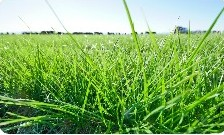
\includegraphics[width=\linewidth,height=3.1cm]{figs/grass_l.jpg}
  \caption*{\footnotesize Left half}
\end{subfigure}\hspace{2pt}
\begin{subfigure}{0.33\textwidth}
  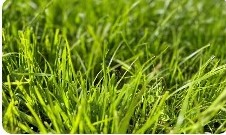
\includegraphics[width=\linewidth,height=3.1cm]{figs/grass_r.jpg}
  \caption*{\footnotesize Right half}
\end{subfigure}
\caption{A pasture photograph holds two adjacent views of one quadrat; the two-stream
architecture exists because of this geometry.}
\label{fig:twostream}
\end{figure}

% ======================================================================
\section{Pasture-biomass model}\label{sec:biomass}

\subsection{Baselines: why ResNet-50 \texorpdfstring{$+$}{+} XGBoost}
We began from the simplest regressors and worked up. Linear and logistic regression on raw pixel
and colour statistics \emph{underfit}---grass is about fine texture and density, which a linear
model on raw features cannot capture. Replacing raw features with a pretrained CNN embedding
transformed the problem, and among backbones a ResNet-50 embedding gave the best trade-off of
representational richness and overfitting on a modest dataset. On top of the embedding, a linear
head could not model the non-linear interactions of the tabular feature vector, whereas
gradient-boosted trees (XGBoost) could. Table~\ref{tab:baselines} summarises the comparison; the
winning pair, \emph{ResNet-50 for features and XGBoost for regression}, became Experiment~A.

\begin{table}[h]
\centering\small
\caption{Baseline comparison for the vision regressor.}
\label{tab:baselines}
\begin{tabular}{p{6.2cm}p{6.0cm}c}
\toprule
\textbf{Approach} & \textbf{What held it back} & \textbf{Verdict}\\
\midrule
Linear / logistic regression on raw pixel \& colour stats & No texture model---grass density is lost & \textcolor{terra}{\textbf{Weak}}\\
ResNet-18 / MobileNet embedding $+$ XGBoost & Lighter backbone loses fine sward detail & Fair\\
VGG-16 embedding $+$ XGBoost & Heavier---overfits our small dataset & Fair\\
ResNet-50 embedding $+$ linear / ridge head & Linear head cannot model tabular interactions & Fair\\
\textbf{ResNet-50 embedding $+$ XGBoost} & Rich 2048-d features $+$ non-linear boosted trees & \textcolor{ochre}{\textbf{Best}}\\
\bottomrule
\end{tabular}
\end{table}

\subsection{Experiment A --- ResNet-50 embedding, green statistics, XGBoost}
The first complete pipeline (Figure~\ref{fig:expA}) uses an ImageNet-pretrained ResNet-50 with its
classifier removed ($\texttt{fc}=\text{Identity}$) as a \emph{frozen} embedding function producing
a 2048-dimensional vector. Beside the embedding, four hand-crafted green statistics are computed
on the raw RGB pixels. One \texttt{XGBRegressor} is trained per target (600 trees, depth 8,
learning rate $0.05$, subsample $0.85$, column subsample $0.85$). Experiment~A established the
three ideas the final model keeps: a pretrained embedding, hand-crafted green statistics beside it,
and a \emph{separate tree model per target}. What it misses is the two-half geometry: the wide
frame is squashed into a single $224\times224$ square.

\begin{figure}[h]
\centering
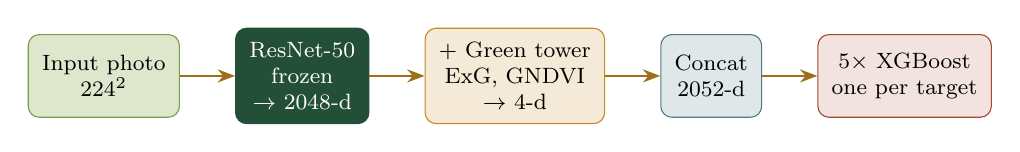
\begin{tikzpicture}[node distance=7mm]
  \node[io] (p) {Input photo\\$224^2$};
  \node[procf,right=of p] (rn) {ResNet-50\\frozen\\$\to$ 2048-d};
  \node[proco,right=of rn] (g) {$+$ Green tower\\ExG, GNDVI\\$\to$ 4-d};
  \node[procs,right=of g] (c) {Concat\\2052-d};
  \node[proct,right=of c] (x) {$5\times$ XGBoost\\one per target};
  \draw[fl] (p)--(rn); \draw[fl] (rn)--(g); \draw[fl] (g)--(c); \draw[fl] (c)--(x);
\end{tikzpicture}
\caption{Experiment A: a frozen ResNet-50 embedding and four green numbers read by five
independent gradient-boosted regressors.}
\label{fig:expA}
\end{figure}

\subsection{Experiment B --- DINO ViT, multi-task head (diverged)}
Experiment~B replaced the backbone with a frozen DINO-pretrained ViT-S/16 ($196$ patch tokens of
dimension $384$), added a learned positional embedding and a four-layer, six-head transformer
encoder, injected the green signal through a cross-attention block and conditioned on the target
name with a $5\times128$ embedding, and attached five task heads (biomass, height, NDVI, species,
state) trained as one weighted MSE/cross-entropy sum. The run \emph{diverged}: a single loss over
quantities on very different scales (grams, centimetres, an index near one), on a frozen backbone
with a freshly initialised transformer, did not stay stable. The lesson---target identity is worth
conditioning on, but a shared neural head is the wrong vehicle---motivates giving each target its
own tree in the final model rather than one fused head.

\subsection{Experiment C --- two-stream DINO, derived targets}
Experiment~C took the left/right geometry seriously. A frozen DINO ViT-S/16 is run twice with
shared weights, once per half; the two $384$-d vectors are concatenated to $768$-d; a head
($768\to512\to3$, GELU, dropout) predicts only the three non-derived targets (clover, dead,
green); and the two sums are obtained afterwards by the physical identities
$\texttt{GDM}=\texttt{green}+\texttt{clover}$ and
$\texttt{Total}=\texttt{GDM}+\texttt{dead}$, with a stratified five-fold ensemble averaged and
clipped at zero. This experiment contributed the two-stream split used by the final model. Its
catch: \texttt{Total} and \texttt{GDM} carry most of the score, yet deriving them by sum lets three
component errors stack in the wrong direction---so the final model learns all five targets
directly.

\subsection{Final architecture}\label{sec:finalarch}
The final model (Figure~\ref{fig:final}) combines the strongest idea of each experiment. Both halves
of the wide photograph pass through \emph{one shared} ResNet-50, giving two 2048-d embeddings.
Twelve hand-crafted green statistics---the four defined below, computed separately on the left half,
the right half and the whole image---are concatenated to form a 4108-d feature vector that five
independent XGBoost regressors read. One photograph produces all five gram values; the networks run
once.

\begin{figure}[h]
\centering
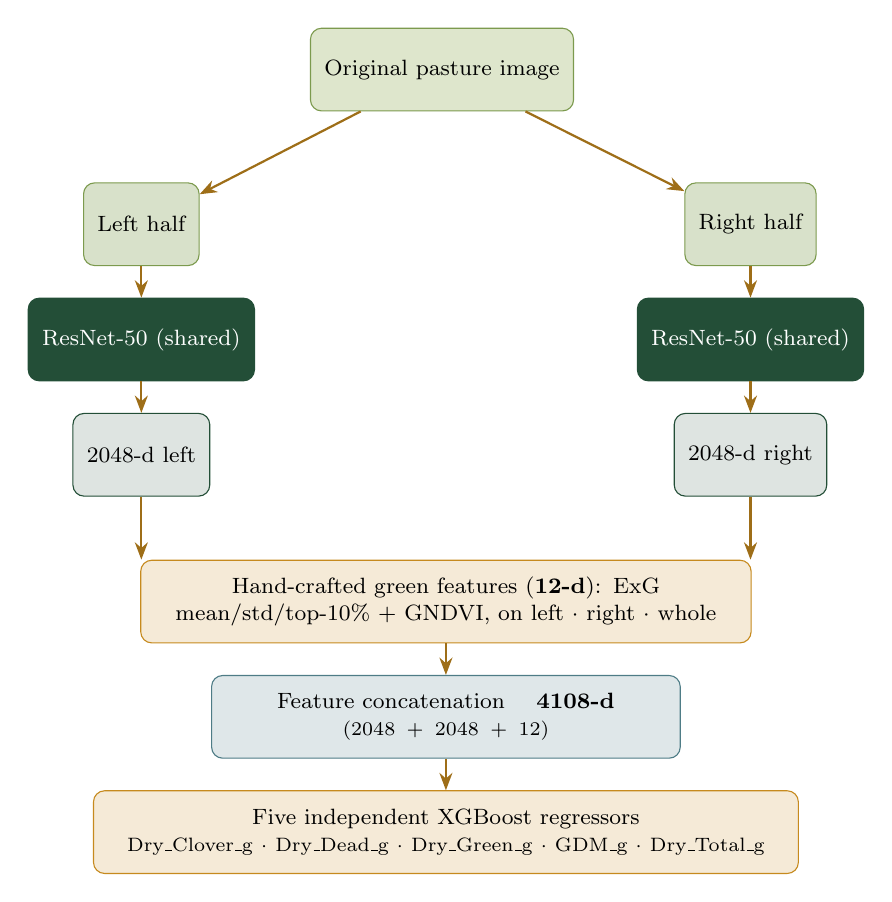
\begin{tikzpicture}[node distance=4mm and 9mm]
  \node[io] (oi) {Original pasture image};
  \node[procm,below left=9mm and 14mm of oi] (lh) {Left half};
  \node[procm,below right=9mm and 14mm of oi] (rh) {Right half};
  \node[procf,below=4mm of lh] (rl) {ResNet-50 (shared)};
  \node[procf,below=4mm of rh] (rr) {ResNet-50 (shared)};
  \node[proc,fill=forest!15,below=4mm of rl] (el) {2048-d left};
  \node[proc,fill=forest!15,below=4mm of rr] (er) {2048-d right};
  \coordinate (mid) at ($(el.south)!0.5!(er.south)$);
  \node[proco,text width=7.4cm,below=8mm of mid,anchor=north] (gf)
     {Hand-crafted green features (\textbf{12-d}): ExG mean/std/top-10\% $+$ GNDVI, on left $\cdot$ right $\cdot$ whole};
  \node[procs,text width=5.6cm,below=4mm of gf] (cc) {Feature concatenation \quad\textbf{4108-d}\\\scriptsize $(2048+2048+12)$};
  \node[proc,fill=ochre!18,draw=ochre,text width=8.6cm,below=4mm of cc] (xg)
     {Five independent XGBoost regressors\\\scriptsize Dry\_Clover\_g $\cdot$ Dry\_Dead\_g $\cdot$ Dry\_Green\_g $\cdot$ GDM\_g $\cdot$ Dry\_Total\_g};
  \draw[fl] (oi)--(lh); \draw[fl] (oi)--(rh);
  \draw[fl] (lh)--(rl); \draw[fl] (rh)--(rr);
  \draw[fl] (rl)--(el); \draw[fl] (rr)--(er);
  \draw[fl] (el.south) -- (el.south |- gf.north);
  \draw[fl] (er.south) -- (er.south |- gf.north);
  \draw[fl] (gf)--(cc); \draw[fl] (cc)--(xg);
\end{tikzpicture}
\caption{Final architecture: a shared two-stream ResNet-50, a 12-d green block, concatenation to
4108-d, and five independent XGBoost regressors.}
\label{fig:final}
\end{figure}

\subsection{The model as mathematics}\label{sec:math}
\textbf{Preprocessing.} Each half is resized to $224^2$ and ImageNet-normalised,
$x_n = (x-\mu)/\sigma$ with $\mu=[0.485,0.456,0.406]$, $\sigma=[0.229,0.224,0.225]$.

\textbf{Shared embedding.} With a frozen, shared ResNet-50 $f_\theta$,
\begin{equation}
e_L = f_\theta(x_L),\qquad e_R = f_\theta(x_R),\qquad e_L,e_R\in\R^{2048}.
\end{equation}

\textbf{Green statistics (raw RGB, $0$--$255$).} With $\mathrm{ExG}=2G-R-B$,
\begin{equation}
g_\bullet = \Big[\ \mathrm{mean}(\mathrm{ExG}),\ \mathrm{std}(\mathrm{ExG}),\
\mathrm{mean}\!\big(\mathrm{ExG}\!\ge\!P_{90}\big),\
\mathrm{mean}\!\Big(\tfrac{G-R}{G+R+\varepsilon}\Big)\ \Big]\in\R^{4},
\end{equation}
computed three times, $g=[\,g_L\mid g_R\mid g_{\text{global}}\,]\in\R^{12}$. ExG mean says
\emph{how green}; its standard deviation, \emph{how uneven}; its top decile, how strong the
greenest tenth (clover and live leaf); and GNDVI is a red/green index needing no near-infrared band.

\textbf{Feature vector.} $\;z=[\,e_L;e_R;g\,]\in\R^{4108}.$

\textbf{Regression.} For each target $t$, a gradient-boosted ensemble of $M$ trees,
\begin{equation}
\hat{y}_t(z)=\sum_{m=1}^{M}\eta\,h_{t,m}(z),\qquad \hat{y}_t\leftarrow\max(\hat{y}_t,0),
\end{equation}
trained to minimise squared error plus regularisation,
\begin{equation}
\mathcal{L}=\sum_i\big(y_i-\hat{y}_i\big)^2+\sum_m\Omega(h_m),\qquad
\Omega(h)=\gamma T+\tfrac12\lambda\lVert w\rVert^2 .
\end{equation}
All five regressors read the same $z$ but do not share trees, so a feature that matters for dead
material is free to be ignored by the clover model. The submission is scored with the weighted
$R^2$ of Equation~\eqref{eq:wr2}.

\subsection{Explainability: Grad-CAM}\label{sec:gradcam}
To check \emph{what} the backbone attends to, we use Gradient-weighted Class Activation Mapping on
the last convolutional block of ResNet-50. For a target output $y^c$ and feature maps $A^k$, the
channel importance is the global-average-pooled gradient
\begin{equation}
\alpha_k^{c}=\frac{1}{Z}\sum_i\sum_j \frac{\partial y^{c}}{\partial A_{ij}^{k}},
\end{equation}
and the localisation map is the ReLU of their weighted combination,
\begin{equation}
L^{c}_{\text{Grad-CAM}}=\mathrm{ReLU}\!\Big(\sum_k \alpha_k^{c}\,A^{k}\Big),
\end{equation}
upsampled to the image and overlaid as a heatmap. ReLU keeps only features that push the output
up. For the biomass backbone this is a sanity check that the embedding attends to vegetation and
not to sky, soil or the quadrat frame; it explains the features and does not change the XGBoost
prediction.

\subsection{From grams to a grazing decision}
The number a farmer can act on is not ``$48$ g'' but ``this paddock can feed these animals for this
many days.'' That conversion is deterministic---not another learned model. With quadrat area
$0.21\,\mathrm{m}^2$ ($70\times30$ cm), a residual left ungrazed, a utilisation fraction and a
daily intake of $2.5\%$ of live weight:
\begin{align}
\text{kg DM/ha} &= \text{grams}\,/\,\text{quadrat area}\times 10,\\
\text{available} &= \max(\text{kg/ha}-\text{residual},0)\times\text{area}\times\text{utilisation},\\
\text{grazing days} &= \text{available}\,/\,(\text{herd}\times\text{liveweight}\times 0.025).
\end{align}
If available feed is zero, the paddock is at or below the residual and should be rested, not grazed.

% ======================================================================
\section{District crop-yield model}\label{sec:yield}

\subsection{The question and the data}
Indian crop statistics are published as production and area for a district, a crop and a season;
dividing gives a yield. This model predicts that \emph{district} yield (tonnes per hectare) for
three crops---rice, maize and wheat---over 33 states and union territories, 645 district names and
the years 1997--2015. It is \emph{not} a forecast of one farmer's field. A prediction for year $Y$
is allowed to see only rows of the same series with \texttt{Crop\_Year} strictly less than $Y$;
using the current year would be leakage. Of $36{,}747$ history rows, $33{,}412$ have at least one
earlier record and are \emph{eligible}; the delivered forest is fitted on all of them.

\subsection{Features and model}
The pipeline has nine inputs: four categories (\texttt{State\_Name}, \texttt{District\_Name},
\texttt{Crop}, \texttt{Season}) one-hot encoded with \texttt{handle\_unknown=ignore}, and five
numbers---\texttt{Crop\_Year}, \texttt{previous\_yield} (the most recent earlier yield), the mean of
the last three earlier yields (\texttt{historical\_mean\_3}), \texttt{years\_since\_previous}, and
\texttt{history\_count}. One-hot encoding yields on the order of $680$ columns even though the user
chooses only a place, crop, season and year. The regressor is a
\texttt{RandomForestRegressor} (scikit-learn 1.6.1): $80$ trees, unlimited depth,
$\texttt{max\_features}=0.7$, minimum two samples to split, minimum three per leaf, bootstrap,
random state $42$. A prediction is the average of the 80 trees, clipped at zero.

\subsection{What the forest actually uses}
Impurity-based importance (Figure~\ref{fig:imp}) shows that about $85\%$ of the split importance
sits on the two features that are just the recent harvests---the three-year mean ($0.624$) and the
previous yield ($0.224$). The year itself is $\sim3\%$ and the gap since the last record under
$1\%$. The forest is therefore a smoothed, slightly adjusted version of the recent district record,
not a crop-growth simulator; a request for a year after 2015 mostly repeats the last known harvests.

\begin{figure}[h]
\centering
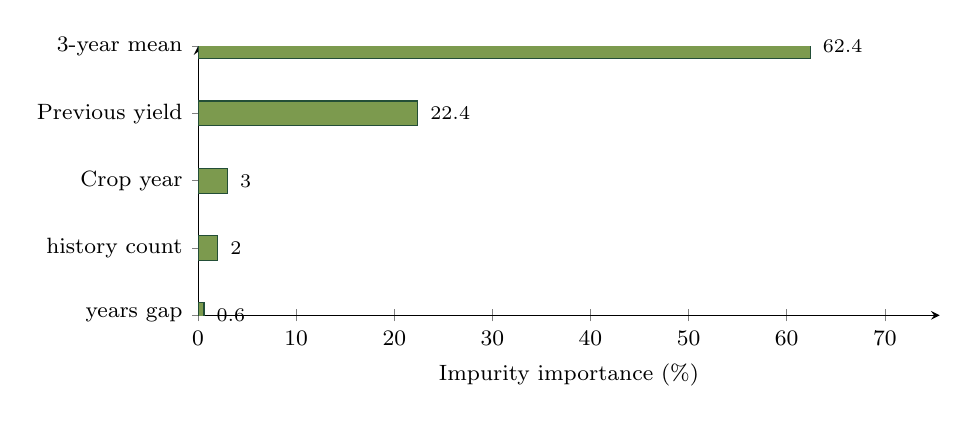
\begin{tikzpicture}
\begin{axis}[
  xbar, width=11cm, height=5.0cm, bar width=9pt,
  xmin=0, xmax=70, enlarge y limits=0.16,
  xlabel={\footnotesize Impurity importance (\%)},
  symbolic y coords={years gap, history count, Crop year, Previous yield, 3-year mean},
  ytick=data, tick label style={font=\footnotesize},
  nodes near coords, nodes near coords style={font=\scriptsize},
  every node near coord/.append style={xshift=1pt},
  axis x line=bottom, axis y line=left,
  xbar legend, enlarge x limits={upper,value=0.08},
]
\addplot[fill=moss,draw=forest] coordinates
  {(0.6,years gap) (2.0,history count) (3.0,Crop year) (22.4,Previous yield) (62.4,3-year mean)};
\end{axis}
\end{tikzpicture}
\caption{Feature importance of the yield forest: the recent harvest record dominates. This is the
figure that stops a ``forecast to 2050'' reading.}
\label{fig:imp}
\end{figure}

\subsection{Evaluation}
Training on the eligible rows before 2015 and testing on the $155$ district--crop--season records of
2015 that also had an earlier year gives the scores in Table~\ref{tab:yield}. Read together: on mean
absolute error the forest does \emph{not} beat ``repeat the recent three-year mean'' (it is worse by
$0.001$ t/ha); on RMSE it is better by $\sim0.022$ t/ha, meaning fewer very large mistakes. A typical
miss is about two-thirds of a tonne per hectare---a large fraction of a normal district yield (median
$1.87$ t/ha). The model is useful as a structured way to read the recent record and to refuse series
with no history; it is not a precise forecast.

\begin{table}[h]
\centering\small
\caption{2015 hold-out scores on 155 district rows (tonnes per hectare).}
\label{tab:yield}
\begin{tabular}{lcc}
\toprule
\textbf{Predictor} & \textbf{MAE} & \textbf{RMSE}\\
\midrule
Baseline: mean of the last three earlier yields & 0.674 & 1.020\\
Random forest (trained on years $<$ 2015) & 0.675 & \textbf{0.998}\\
\bottomrule
\end{tabular}
\end{table}

% ======================================================================
\section{Soil-profile model}\label{sec:soil}

\subsection{The question and the data}
A soil test returns six numbers; the model says which group of previously seen tests it most
resembles and shows that group's typical values. It does \emph{not} name a soil type, grade
fertility or compute a fertiliser dose. The data is the AgriNet soil-fertility table
(DOI \href{https://doi.org/10.17632/c7tr9j78td.1}{10.17632/c7tr9j78td.1}, CC BY 4.0), $257$ samples
from Bareilly district, Uttar Pradesh---one district, so a held-out slice is not geographic
validation, a limit the product states on every card.

\subsection{Scaling and model}
The six measurements---pH, EC (millimhos/cm), organic carbon (\%), and N, P, K (kg/ha)---do not
share a scale, so a \texttt{StandardScaler} fitted on the 257 rows maps each to zero mean and unit
variance before $k$-means, which uses Euclidean distance. A search over the number of groups
(Table~\ref{tab:sil}) peaks at four clusters by training silhouette; a separate held-out silhouette
of $0.556$ confirms moderate, overlapping separation. The delivered \texttt{KMeans} uses the Lloyd
algorithm, $20$ initialisations, $300$ maximum iterations and random state $42$.

\begin{table}[h]
\centering\small
\begin{minipage}[t]{0.46\textwidth}
\centering
\caption{Silhouette search over $k$.}
\label{tab:sil}
\begin{tabular}{cccc}
\toprule
$k$ & Silhouette & Smallest & Largest\\
\midrule
2 & 0.514 & 89 & 116\\
3 & 0.568 & 29 & 116\\
\textbf{4} & \textbf{0.634} & 29 & 76\\
5 & 0.605 & 27 & 76\\
\bottomrule
\end{tabular}
\end{minipage}\hfill
\begin{minipage}[t]{0.5\textwidth}
\centering
\caption{Assignment of a new test.}
\label{tab:soilsteps}
\begin{tabular}{p{7.4cm}}
\toprule
1. Order the six numbers (pH, EC, OC, N, P, K).\\
2. Scale with the saved mean and std.\\
3. Euclidean distance to each of four centres.\\
4. Nearest centre is the cluster.\\
5. Flag if that distance $>1.260$ (95th pct).\\
\bottomrule
\end{tabular}
\end{minipage}
\end{table}

\subsection{The four groups}
Cluster identifiers are arbitrary---they are \emph{not} ordered from best to worst soil
(Table~\ref{tab:clusters}). Interpretation is by comparing a test to the group medians. Because pH
on this dataset has a standard deviation of only $0.20$, even a moderate pH change is a long step in
scaled space, so a genuinely acidic (non-Bareilly) soil is often flagged---the model telling the
truth about its training geography.

\begin{table}[h]
\centering\small
\caption{The four soil-profile clusters (medians in original units).}
\label{tab:clusters}
\begin{tabular}{llccl}
\toprule
\textbf{Cluster} & \textbf{Samples} & \textbf{pH} & \textbf{N\,$\cdot$\,P\,$\cdot$\,K} & \textbf{Character}\\
\midrule
Cluster 0 & 99 & 7.21 & 105 $\cdot$ 4.5 $\cdot$ 125 & Near-neutral, low salts, very low phosphorus\\
Cluster 1 & 68 & 6.91 & 143 $\cdot$ 15 $\cdot$ 167 & Slightly acidic, higher N and P\\
Cluster 2 & 30 & 6.81 & 167 $\cdot$ 9 $\cdot$ 257 & Lower pH, high salinity, highest OC/N/K\\
Cluster 3 & 60 & 7.26 & 72 $\cdot$ 15 $\cdot$ 93 & Slightly alkaline, lowest OC/N/K\\
\bottomrule
\end{tabular}
\end{table}

% ======================================================================
\section{The AgriAssist agentic platform}\label{sec:agent}

\subsection{System shape}
A phone browser (React~19, Vite, Tailwind, Clerk session) calls a FastAPI backend over HTTPS with a
Clerk JWT on every request. The backend hosts a LangGraph agent whose single turn is the graph
\[
\textsf{START}\;\to\;\textsf{load\_context}\;\to\;\textsf{agent}\;\rightleftarrows\;\textsf{tools}\;\to\;\textsf{END}.
\]
\texttt{load\_context} loads the farm profile, the long-term summary and recent chat summaries;
\texttt{agent} is a tool-calling LLM with vision (xAI Grok by default; Google Gemini, NVIDIA NIM or
Meta Muse selectable). Parallel tool calls run together and the loop stops when the agent answers
with no tool call. The user id comes from the verified token server-side, so the model cannot read
another farm. Memory reflection runs \emph{after} the answer is streamed, so it never adds latency.

\subsection{The twelve tools}
The three trained models are exposed as agent tools alongside live data and memory tools:
\texttt{predict\_pasture\_biomass}, \texttt{diagnose\_plant\_disease} (a constrained vision call),
\texttt{predict\_crop\_yield}, \texttt{describe\_soil\_profile}, \texttt{estimate\_grazing\_days}
(the deterministic conversion), \texttt{get\_mandi\_prices} (Agmarknet, web fallback),
\texttt{get\_weather} (Open-Meteo), \texttt{web\_search}, \texttt{remember\_fact},
\texttt{recall\_memories}, \texttt{search\_past\_conversations} and \texttt{update\_farm\_profile}.
There is no separate crop-recommender model and no livestock-health model.

\subsection{Three-tier memory}
Memory is designed to behave like a person who knows a farmer, not a log of every sentence.
\emph{Session} memory is the full message list of a chat (LangGraph Postgres checkpointer, last 24
messages sent verbatim). \emph{Short-term} memory is a title and 2--4 sentence summary of each chat.
\emph{Long-term} memory is \emph{one} prose summary ($\sim120$ words) plus the structured farm
profile. A fact becomes long-term only by two doors: the person asks, or the system notices it in
two distinct chats; weather, prices, today's problem and tool results are never stored. Promotion
rewrites the single summary rather than appending to a growing list. Embeddings are local
(\texttt{fastembed}, multilingual MiniLM, 384-d), so a Hindi memory and an English query can match.

\subsection{Voice and language}
The agent replies in the language and script of the latest message; interface language is a separate
setting. Sarvam Saaras v3 provides speech-to-text in 22 Indian languages and Bulbul v3
text-to-speech in 11, with a hands-free voice mode that begins speaking at the first finished
sentence. Anything the person typed is never translated; enumerated choices (farmer, acre, wheat)
are shown translated but stored in canonical English.

% ======================================================================
\section{Discussion and limitations}
Each model is deliberately honest about what it is not. The biomass model takes only the photograph
and reports grams per quadrat; converting to a paddock decision assumes a residual and a utilisation
that must be stated. The yield forest is a smoothed reading of the recent district record, with a
typical error near $0.67$ t/ha and no real extrapolation past 2015. The soil clusterer describes
similarity to $257$ Bareilly samples and flags tests that are unlike them; it is not a fertility
grade or a dose. Surfacing these limits---in the report, and on every result card in the
product---is part of the design, not an afterthought.

\section{Conclusion and future work}
AgriAssist answers the CSIRO pasture-biomass problem with a two-stream ResNet-50 and five
gradient-boosted regressors reached through three documented experiments, and situates it beside a
district crop-yield forest and a soil-profile clusterer inside one agent that remembers the farm and
answers in the farmer's language. Future work includes WhatsApp access, proactive weather and price
alerts, a government-scheme finder from the profile, and Sentinel-2 NDVI of the user's field
alongside the biomass model.

% ======================================================================
\begin{thebibliography}{9}
\small
\bibitem{csiro} Commonwealth Scientific and Industrial Research Organisation (CSIRO).
  \emph{Pasture Biomass Challenge}. \url{https://www.csiro.au}; competition:
  \url{https://www.kaggle.com/competitions/csiro-biomass}.
\bibitem{resnet} K.~He, X.~Zhang, S.~Ren, J.~Sun. Deep Residual Learning for Image Recognition.
  \emph{CVPR}, 2016.
\bibitem{xgboost} T.~Chen, C.~Guestrin. XGBoost: A Scalable Tree Boosting System. \emph{KDD}, 2016.
\bibitem{dino} M.~Caron \emph{et al.} Emerging Properties in Self-Supervised Vision Transformers
  (DINO). \emph{ICCV}, 2021.
\bibitem{gradcam} R.~R.~Selvaraju \emph{et al.} Grad-CAM: Visual Explanations from Deep Networks via
  Gradient-based Localization. \emph{ICCV}, 2017.
\bibitem{rf} L.~Breiman. Random Forests. \emph{Machine Learning}, 45(1), 2001.
\bibitem{sklearn} F.~Pedregosa \emph{et al.} Scikit-learn: Machine Learning in Python.
  \emph{JMLR}, 12, 2011.
\bibitem{agrinet} A.~S.~Atul. \emph{AgriNet soil-fertility dataset}, Bareilly, India.
  DOI \href{https://doi.org/10.17632/c7tr9j78td.1}{10.17632/c7tr9j78td.1}, CC BY 4.0.
\bibitem{langgraph} LangChain. \emph{LangGraph}: stateful, multi-actor LLM applications.
  \url{https://github.com/langchain-ai/langgraph}.
\end{thebibliography}

\end{document}
